\documentclass[letter,12pt,sffamily]{article}
\usepackage{datetime}
\usepackage{tikz}
\usepackage{algorithm}
\usepackage{csquotes}
\usepackage{amsmath}
\usepackage[noend]{algpseudocode}
\usepackage{fontspec}
\usepackage{minted}
\usemintedstyle[c]{tango}
\usepackage{listings}
\usetikzlibrary{trees}
\makeatletter
\def\BState{\State\hskip-\ALG@thistlm}
\makeatother

\begin{document}
\tikzstyle{every node}=[thick,anchor=west, rounded corners, font={\scriptsize\ttfamily}, inner sep=2.5pt]
\tikzstyle{selected}=[draw=blue,fill=blue!10]
\tikzstyle{root}=[selected, fill=blue!30]

\begin{titlepage}
  \begin{center}
    \vspace*{1cm}
    \Huge
    \textbf{Chapter 6}\\
    \vspace{0.5cm}
    \LARGE
    Pipes and the Client-Server Model
    \vfill
    \Large
    \textbf{Jonathan Reyna}\\
    College of Engineering and Computing\\
    Nova Southeastern University\\
    \usdate{\today}
  \end{center}
\end{titlepage}
\tableofcontents
\pagebreak
\section{Program 6.7: pipeserver}
\mintinline{c}{pipeserver} demonstrates a simple use case of a pipe, while embracing the client-server model. The pipe server listens, just as a web or tcp server would, for data written to it. As data is written to the pipe, it is forwarded to the standard output file descriptor. That output is then redirected to a log file for later examination.
\subsection{Relation to Learned Material}
Pipes are the oldest method of IPC on UNIX systems, and satisfy the frequent requirement that output from one command, must be input to another. This idea translates to processes as well. FIFOs
are a variation on pipes. A FIFO differs, in that it can be used to communicate between any processes.
Chapter 6 discusses the various UNIX special files, and their practial uses in applications. It also introduces the client-server model. Program 6.7 combines these concepts.
\subsection{Source Code}
The following source will be compiled to produce the \mintinline{c}{pipeserver} program.
\renewcommand{\theFancyVerbLine}{
\sffamily\textcolor[rgb]{0.5,0.5,0.5}{\scriptsize\arabic{FancyVerbLine}}}

\begin{minted}[mathescape,
    linenos,
    numbersep=5pt,
    gobble=0,
    frame=lines,
  framesep=2mm]{c}

#include <errno.h>
#include <fcntl.h>
#include <stdio.h>
#include <unistd.h>
#include <sys/stat.h>
#include "../restart/restart.h"

#define FIFOARG 1
#define FIFO_PERMS (S_IRWXU | S_IWGRP | S_IWOTH)

int main(int argc, char *argv[]) {
  int requestfd;

  /* name of server fifo is passed on the command line */
  if (argc != 2) { 
    fprintf(stderr, "Usage: %s fifoname > logfile\n", argv[0]);
    return 1;
  }
	
  /* int mkfifo(const char *pathname, mode_t mode); */
  /* Create a new FIFO named PATH,                  */ 
  /* with permission bits MODE.                     */
  if ((mkfifo(argv[FIFOARG], FIFO_PERMS) == -1) && 
      (errno != EEXIST)) {
    perror("Server failed to create a FIFO");
    return 1;
  }
	
  /* open a read/write communication endpoint to the pipe */
  if ((requestfd = open(argv[FIFOARG], O_RDWR)) == -1) {
    perror("Server failed to open its FIFO");
    return 1;
  }
  copyfile(requestfd, STDOUT_FILENO);
  return 1;
}
\end{minted}
\subsection{Environment}
The operating system environment used to demonstrate \mintinline{c}{pipeserver} will be Linux Mint 17.2.
\begin{figure}[H]
	\centering
	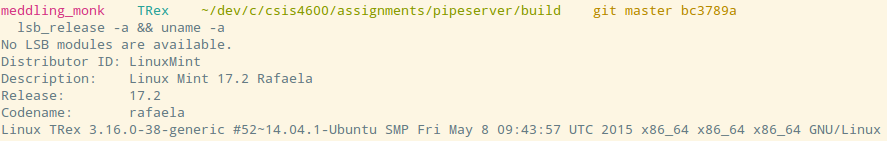
\includegraphics[width=1\linewidth]{./images/0}
	\caption[env]{Build Environment}
	\label{fig:0}
\end{figure}
\subsection{Build}
The CMake metabuild system will be used to create native UNIX Makefiles. 
\begin{figure}[H]
	\centering
	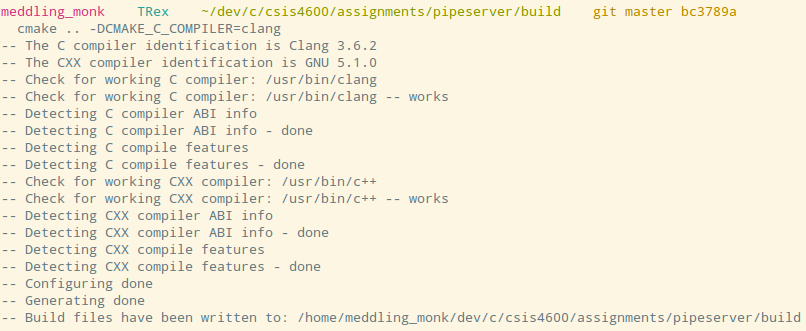
\includegraphics[width=1\linewidth]{./images/1}
	\caption[CMake_prep]{CMake Metabuild}
	\label{fig:1}
\end{figure}
Those makefiles are executed to build and link the final executable.
\begin{figure}[H]
	\centering
	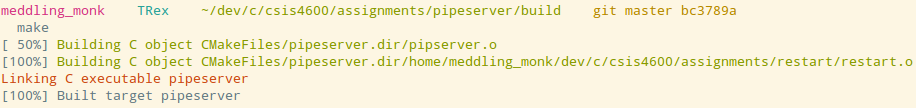
\includegraphics[width=1\linewidth]{./images/2}
	\caption[make_build]{UNIX make}
	\label{fig:2}
\end{figure}
\subsection{Run}
To demonstrate \mintinline{c}{pipeserver}, it will be loaded into GDB. The pipe's output will be redirected to a file called \mintinline{bash}{test.log}.
\begin{figure}[H]
	\centering
	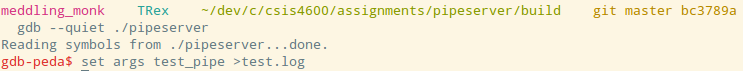
\includegraphics[width=1\linewidth]{./images/3}
	\caption[starting_GDB]{GNU Project Debugger initialization}
	\label{fig:3}
\end{figure}
The \mintinline{c}{mkfifo()} system call will be used to create the FIFO. If it returns -1, an error occurred, and the program must exit. 
\begin{figure}[H]
	\centering
	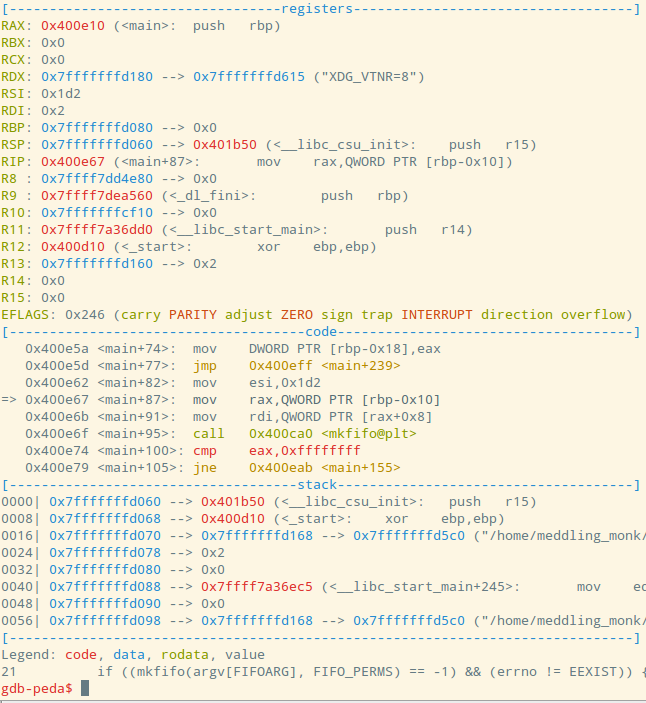
\includegraphics[width=1\linewidth]{./images/4}
	\caption[mkfifo_error_check]{\mintinline{c}{mkfifo()} error check}
	\label{fig:4}
\end{figure}
Since the program has reached this point, there was no error creating the FIFO, and the FIFO can now be opened. The new
FIFO's file descriptor will be assigned to \mintinline{c}{requestfd}. This assignemnt can be verified by printing its value with GDB.
\begin{figure}[H]
	\centering
	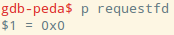
\includegraphics[width=0.3\linewidth]{./images/5}
	\caption[requestfd_val_check_1]{First \mintinline{c}{requestfd} value check}
	\label{fig:5}
\end{figure}
Moving to the next instruction in GDB has shown that \mintinline{c}{open()} executed successfully. The program is now ready to copy everything from \mintinline{c}{requestfd} to \mintinline{c}{STDOUT_FILENO}.
\begin{figure}[H]
	\centering
	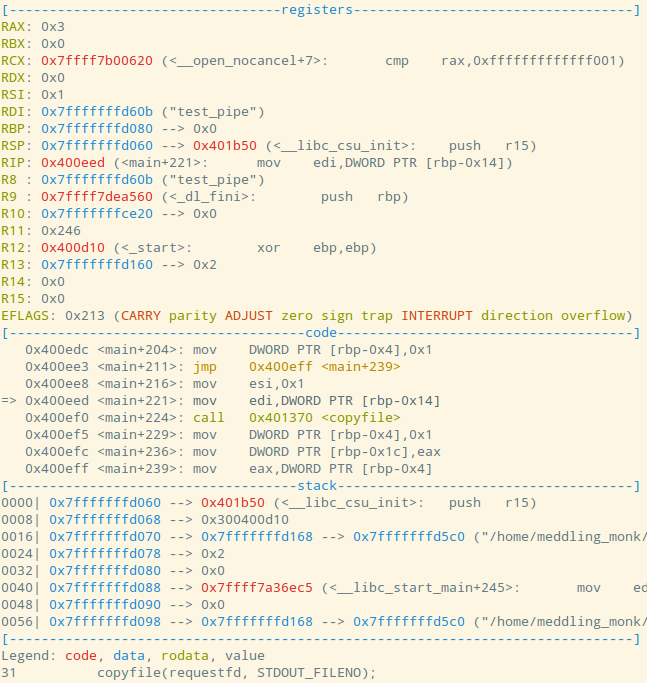
\includegraphics[width=1\linewidth]{./images/6}
	\caption[copyfile]{Copy input from \mintinline{c}{requestfd} to the standard out file descriptor}
	\label{fig:6}
\end{figure}
Using GDB to print the \mintinline{c}{requestfd} file descriptor value, it can be shown that it was assigned a value of 3.
\begin{figure}[H]
	\centering
	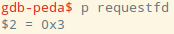
\includegraphics[width=0.3\linewidth]{./images/7}
	\caption[requestfd_val_check_2]{Second \mintinline{c}{requestfd} value check}
	\label{fig:7}
\end{figure}
The recently created pipe can be viewed with \mintinline{bash}{ls}, and its type can be observed by the 'p' leading the permission mask. 
\begin{figure}[H]
	\centering
	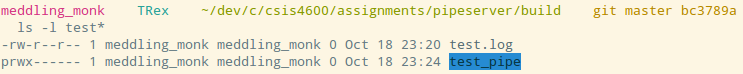
\includegraphics[width=1\linewidth]{./images/8}
	\caption[created_files_listing]{Listing of files created by the \mintinline{c}{pipeserver} process}
	\label{fig:8}
\end{figure}
To see the output of \mintinline{c}{pipeserver} in real time, this example will use the UNIX \mintinline{bash}{tail} command, with the \mintinline{bash}{-f} option to follow the output appended data as the file grows.
\begin{figure}[H]
	\centering
	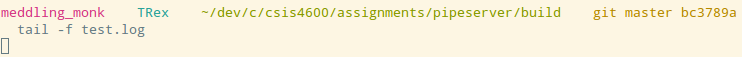
\includegraphics[width=1\linewidth]{./images/9}
	\caption[tailf]{Monitoring \mintinline{bash}{test.log} with \mintinline{bash}{tail -f}}
	\label{fig:9}
\end{figure}
Demonstrating the \mintinline{c}{pipeserver} will require data to be written to the pipe it is listening to. This example will redirect the following quote, by Edward V. Berard to the FIFO:
\enquote{Walking on water and developing software from a specification are easy if both are frozen.}
\begin{figure}[H]
	\centering
	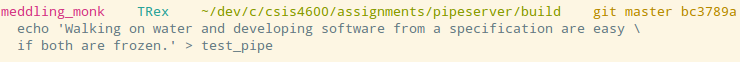
\includegraphics[width=1\linewidth]{./images/10}
	\caption[text_redirection]{Redirection of echoed text to the pipe}
	\label{fig:10}
\end{figure}
Refocusing attention to the \mintinline{bash}{tail} command running against \mintinline{bash}{test.log}, the quoted text can be seen printed to the terminal. This confirms that the \mintinline{c}{pipeserver} read and wrote the text
that was sent to it successfully.
\begin{figure}[H]
	\centering
	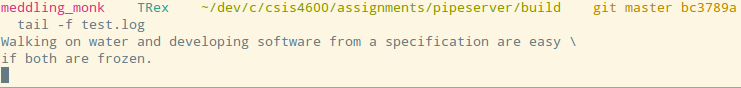
\includegraphics[width=1\linewidth]{./images/11}
	\caption[tail_pipe_follow]{Results from \mintinline{bash}{tail}'s pipe follow}
	\label{fig:11}
\end{figure}
This brings \mintinline{c}{pipeserver}'s demonstration to a successful conclusion. However ending the process will require some force, since \mintinline{c}{pipeserver} is in an infinite loop with \mintinline{c}{copyfile()}.
To end the program, it will require sending a \mintinline{c}{SIGINT}, or interrupt signal, to the process.
\begin{figure}[H]
	\centering
	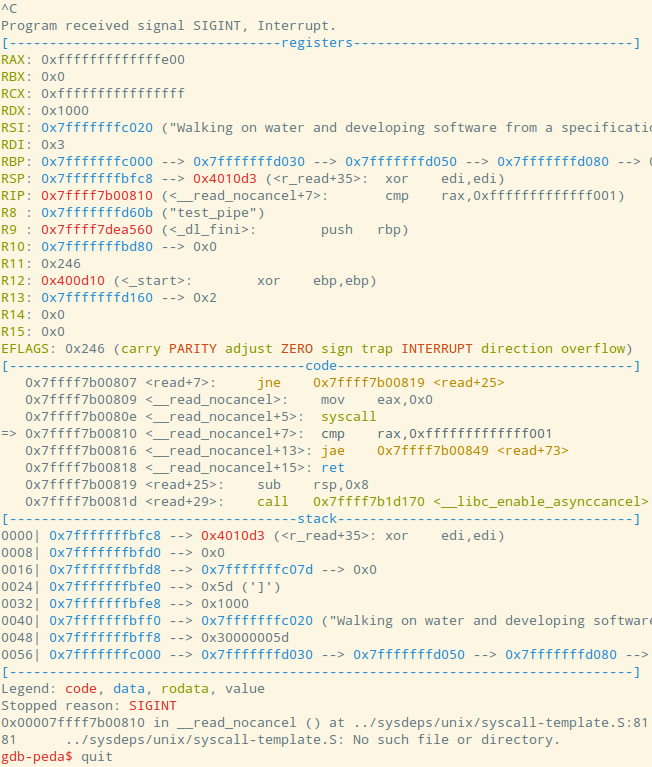
\includegraphics[width=1\linewidth]{./images/12}
	\caption[sigint]{End the \mintinline{c}{pipeserver} process}
	\label{fig:12}
\end{figure}
\section{Program 6.8: pipeclient}
\mintinline{c}{pipeclient} uses \mintinline{c}{pipeserver}. It demonstrates how FIFOs can be used for IPC. In this case, \mintinline{c}{pipeclient} will write its PID, and the current time to the FIFO.
Upon completion, \mintinline{c}{pipeclient} will close the FIFO's file descriptor, and return 0 indicating successful execution to the shell.
\subsection{Relation to Learned Material}
This program completes the demonstration of the client/server model talked about in the book. It takes the client side, where the previous program took the server side.
\subsection{Source Code}
The following source will be compiled to produce the \mintinline{c}{pipeclient} program.
\renewcommand{\theFancyVerbLine}{
	\sffamily\textcolor[rgb]{0.5,0.5,0.5}{\scriptsize\arabic{FancyVerbLine}}}

\begin{minted}[mathescape,
	linenos,
	numbersep=5pt,
	gobble=0,
	frame=lines,
	framesep=2mm]{c}
	
#include <fcntl.h>
#include <stdio.h>
#include <stdlib.h>
#include <time.h>
#include <unistd.h>
#include <linux/limits.h>
#include <string.h>
#include "../restart/restart.h"

#define FIFOARG 1

int main(int argc, char *argv[]) {
  char requestbuf[PIPE_BUF];
  int requestfd;
	
  if (argc != 2) {
    fprintf(stderr, "Usage: %s fifoname", argv[0]);
    return 1;
  }
	
  if ((requestfd = open(argv[FIFOARG], O_WRONLY)) == -1) {
    perror("Client failed to open log fifo for writing");
    return 1;
  }
	
  time_t curtime = time(NULL);
  snprintf(requestbuf, PIPE_BUF, "%d: %s", (int) getpid(), 
           ctime(&curtime));
  int len = strlen(requestbuf);
	
  if (r_write(requestfd, requestbuf, len) != len) {
    perror("Client failed to write");
    return 1;
  }
	
  r_close(requestfd);
	
  return 0;
}
\end{minted}
\subsection{Environment}
The operating system environment used to demonstrate \mintinline{c}{pipeclient} will be Linux Mint 17.2.
\begin{figure}[H]
	\centering
	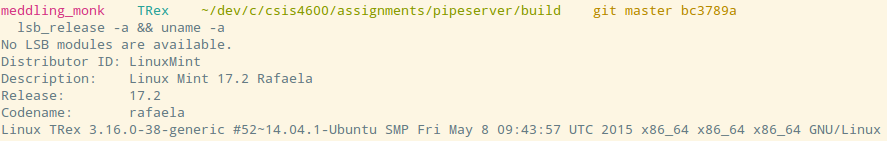
\includegraphics[width=1\linewidth]{./images/0}
	\caption[env]{Build Environment}
	\label{fig:13}
\end{figure}
\subsection{Build}
The CMake metabuild system will be used to create native UNIX Makefiles. 
\begin{figure}[H]
	\centering
	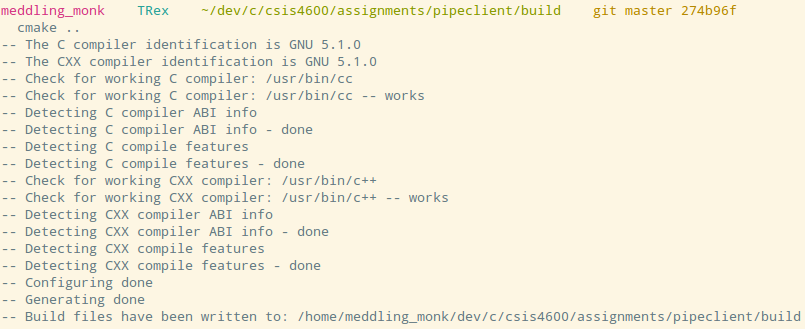
\includegraphics[width=1\linewidth]{./images/13}
	\caption[CMake_prep]{CMake Metabuild}
	\label{fig:14}
\end{figure}
Those makefiles are executed to build and link the final executable.
\begin{figure}[H]
	\centering
	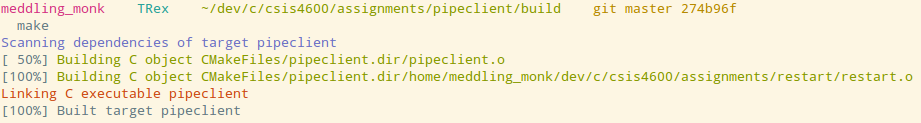
\includegraphics[width=1\linewidth]{./images/14}
	\caption[make_build]{UNIX make}
	\label{fig:15}
\end{figure}
\subsection{Run}
To demonstrate \mintinline{c}{pipeclient}, and the client/server model, this example will begin by starting the \mintinline{c}{pipeserver} previously demonstrated.
It will be executed as a background process to avoid interference with further use of the terminal.
\begin{figure}[H]
	\centering
	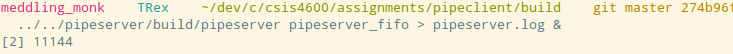
\includegraphics[width=1\linewidth]{./images/15}
	\caption[starting_pipe_server]{Starting the pipe server}
	\label{fig:16}
\end{figure}
Now \mintinline{c}{pipeclient} will be loaded into GDB, and the program arguments will be set to use the FIFO created by \mintinline{c}{pipeserver}.
\begin{figure}[H]
	\centering
	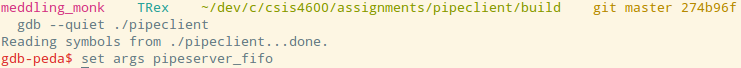
\includegraphics[width=1\linewidth]{./images/16}
	\caption[preparing_gdb]{Preparing GDB}
	\label{fig:17}
\end{figure}
After \mintinline{c}{pipeclient} verifies that it has been executed with the correct number of arguments, it opens the FIFO, and returns
the corresponding file descriptor. The permissions are set on the FIFO to open it for writing only.
\begin{figure}[H]
	\centering
	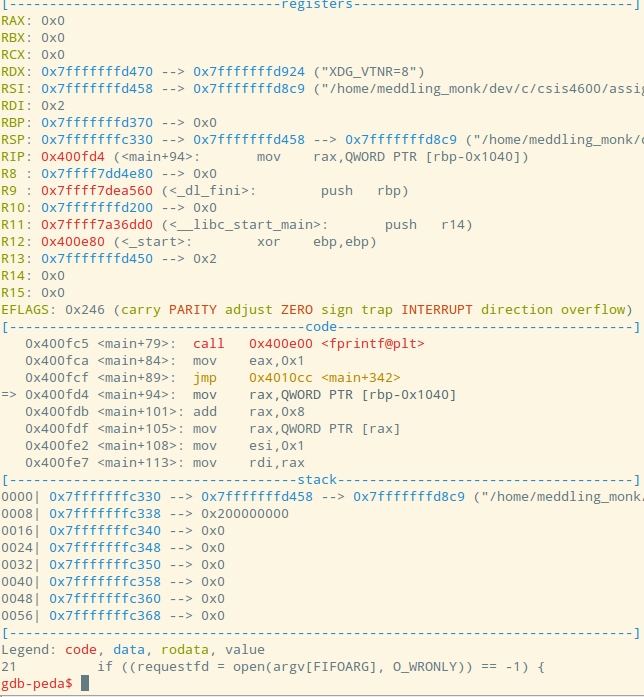
\includegraphics[width=1\linewidth]{./images/17}
	\caption[opening_fifo]{Opening the FIFO for writing}
	\label{fig:18}
\end{figure}
Subsequent to the \mintinline{c}{open()} instruction, the file descriptor for the FIFO can be printed using GDB.
\begin{figure}[H]
	\centering
	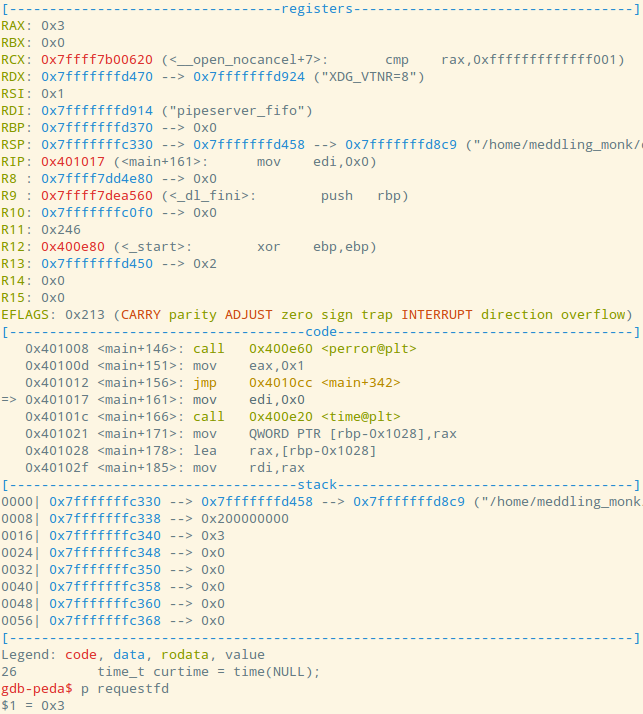
\includegraphics[width=1\linewidth]{./images/18}
	\caption[assigned_file_descriptor]{Checking the assigned file descriptor}
	\label{fig:19}
\end{figure}
Here, the request buffer will be printed. It will allow for verification later, when compared with what was written to the \mintinline{c}{pipeserver} log.
It should also be noted that the contents of the buffer can be clearly seen on the stack at address \mintinline{c}{0x7fffffffc348}. The request file descriptor
is located on the stack at \mintinline{c}{0x7fffffffc340}.
\begin{figure}[H]
	\centering
	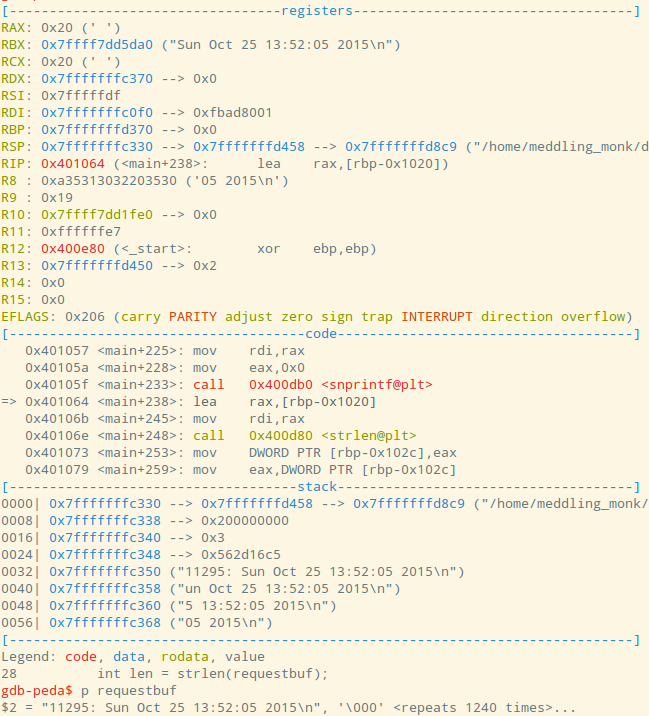
\includegraphics[width=1\linewidth]{./images/19}
	\caption[printing_buffer]{Printing the buffer before writing}
	\label{fig:20}
\end{figure}
Finally, the pipeserver log can be checked against what \mintinline{c}{pipeclient} wrote. 
\begin{figure}[H]
	\centering
	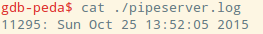
\includegraphics[width=.5\linewidth]{./images/20}
	\caption[verifying_pipeserver_read]{Verifying the \mintinline{c}{pipeserver}'s read}
	\label{fig:21}
\end{figure}
For completeness, \mintinline{c}{pipeclient}'s PID can be verified with GDB, and it will show that the PID printed there, will match what was written to \mintinline{c}{pipeserver}'s log.
\begin{figure}[H]
	\centering
	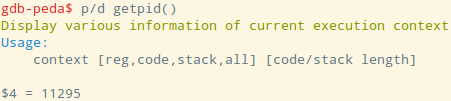
\includegraphics[width=.7\linewidth]{./images/21}
	\caption[verifying_write_from_current_pid]{Verifying the write was from this process}
	\label{fig:22}
\end{figure}
\section{Programs 6.9 and 6.10: seqserverbad and seqclientbad}
The textbook describes program 6.9, the sequence server, as a program that \blockquote{reads a character from the request pipe, and transmits a sequence number to the sequence pipe.} It describes the sequence client as a program that \blockquote{writes requests to a pipe and reads the sequence number from the sequence pipe.} It 
specifically notes that the client, in this case, can cause the server to exit. This is unusual, since most modern servers do not allow the client to have this level
of control.
\subsection{Relation to Learned Material}
These programs demonstrate the client/server model, and help introduce some of the problems related to the lack of atomicity with pipe reads.
\subsection{Source Code}
Both the \mintinline{c}{seqserverbad} and \mintinline{c}{seqclientbad} programs' source can be found in this section.
\subsubsection{seqserverbad}
\renewcommand{\theFancyVerbLine}{
	\sffamily\textcolor[rgb]{0.5,0.5,0.5}{\scriptsize\arabic{FancyVerbLine}}}

\begin{minted}[mathescape,
	linenos,
	numbersep=5pt,
	gobble=0,
	frame=lines,
	framesep=2mm]{c}
	

#include <errno.h>
#include <fcntl.h>
#include <stdio.h>
#include <unistd.h>
#include <sys/stat.h>
#include "../restart/restart.h"

#define ERROR_CHAR 'e'
#define OK_CHAR 'g'
#define REQUEST_FIFO 1
#define REQ_PERMS (S_IRUSR | S_IWUSR | S_IWGRP | S_IWOTH)
#define SEQUENCE_FIFO 2
#define SEQ_PERMS (S_IRUSR | S_IWUSR | S_IRGRP | S_IROTH)

int main(int argc, char *argv[]) {
  char buf[1];
  int reqfd, seqfd;
  long seqnum = 1;
  if (argc != 3) {
    fprintf(stderr, "Usage: %s requestfifo sequencefifo\n", argv[0]);
    return 1;
  }
	
  if ((mkfifo(argv[REQUEST_FIFO], REQ_PERMS) == -1) && (errno != EEXIST)) {
    perror("Server failed to create request FIFO");
    return 1;
  }
	
  if ((mkfifo(argv[SEQUENCE_FIFO], SEQ_PERMS) == -1) && errno != EEXIST) {
    perror("Server failed to create sequence FIFO");
    if (unlink(argv[REQUEST_FIFO]) == -1)
    perror("Server failed to unlinik request FIFO");
    return 1;
  }
	
  if (((reqfd = open(argv[REQUEST_FIFO], O_RDWR)) == -1) ||
     ((seqfd = open(argv[SEQUENCE_FIFO], O_RDWR)) == -1)) {
    perror("Server failed to open one of the FIFOs");
    return 1;
  }
	
  for (; ;) {
    if (r_read(reqfd, buf, 1) == 1) {
      if ((buf[0] == OK_CHAR) &&
      (r_write(seqfd, &seqnum, sizeof(seqnum)) == sizeof(seqnum))) {
        seqnum++;
      }
      else if (buf[0] == ERROR_CHAR) {
        break;
      }
    }
  }
	
  if (unlink(argv[REQUEST_FIFO]) == -1) {
    perror("Server failed to unlink request FIFO");
  }
  if (unlink(argv[SEQUENCE_FIFO]) == -1) {
    perror("Server failed to unlink sequence FIFO");
  }
	
  return 0;
}
\end{minted}
\subsubsection{seqclientbad}
\renewcommand{\theFancyVerbLine}{
	\sffamily\textcolor[rgb]{0.5,0.5,0.5}{\scriptsize\arabic{FancyVerbLine}}}

\begin{minted}[mathescape,
	linenos,
	numbersep=5pt,
	gobble=0,
	frame=lines,
	framesep=2mm]{c}
	
	
#define _XOPEN_SOURCE

#include <fcntl.h>
#include <stdio.h>
#include <stdlib.h>
#include <unistd.h>
#include "../restart/restart.h"

#define ERROR_CHAR 'e'
#define OK_CHAR 'g'
#define REPEAT_MAX 100
#define REQUEST_FIFO 1
#define SEQUENCE_FIFO 2
#define SLEEP_MAX 5

int main(int argc, char *argv[]) {
  int i;
  char reqbuf[1];
  int reqfd, seqfd;
  long seqnum;

  if (argc != 3) {
    fprintf(stderr, "Usage: %s requestfifo sequencefifo\n", argv[0]);
    return 1;
  }

  if ((reqfd = open(argv[REQUEST_FIFO], O_WRONLY)) == -1 ||
     ((seqfd = open(argv[SEQUENCE_FIFO], O_RDONLY)) == -1)) {
    perror("Client failed to open a FIFO");
    return 1;
  }
  
  for (i = 0; i < REPEAT_MAX; i++) {
    reqbuf[0] = OK_CHAR;
    sleep((int) (SLEEP_MAX * drand48()));
    
    if (r_write(reqfd, reqbuf, 1) == -1) {
      perror("Client failed to write request");
      break;
    }
	
    if (r_read(seqfd, &seqnum, sizeof(seqnum)) != sizeof(seqnum)) {
      fprintf(stderr, "Client failed to read full sequence number\n");
      reqbuf[0] = ERROR_CHAR;
      r_write(reqfd, reqbuf, 1);
      break;
    }

    fprintf(stderr, "[%ld]:received sequence number %ld\n",
           (long) getpid(), seqnum);
  }
	
  return 0;
}
\end{minted}
\subsection{Environment}
The operating system environment used to demonstrate \mintinline{c}{seqserverbad} and \mintinline{c}{seqclientbad} will be Linux Mint 17.2.
\begin{figure}[H]
	\centering
	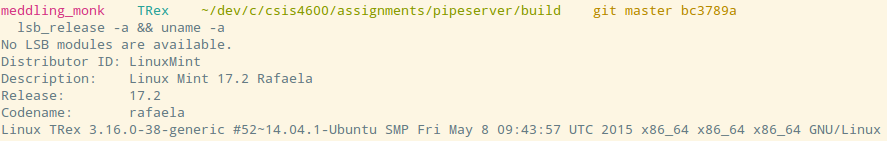
\includegraphics[width=1\linewidth]{./images/0}
	\caption[env]{Build Environment}
	\label{fig:23}
\end{figure}
\subsection{Build}
Both builds will use CMake and UNIX makefiles.
\subsubsection{seqserverbad}
\begin{figure}[H]
	\centering
	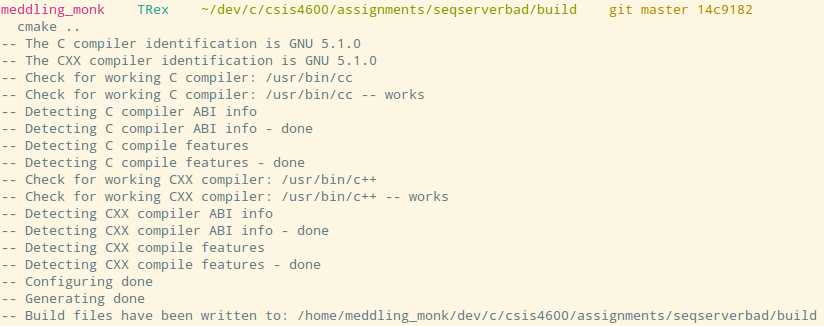
\includegraphics[width=1\linewidth]{./images/22}
	\caption[seqserverbad_cmake_prep]{\mintinline{c}{seqserverbad} CMake Metabuild}
	\label{fig:24}
\end{figure}
\begin{figure}[H]
	\centering
	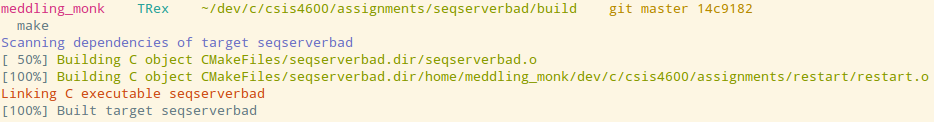
\includegraphics[width=1\linewidth]{./images/23}
	\caption[seqserverbad_make_build]{\mintinline{c}{seqserverbad} UNIX make}
	\label{fig:25}
\end{figure}
\subsubsection{seqclientbad}
\begin{figure}[H]
	\centering
	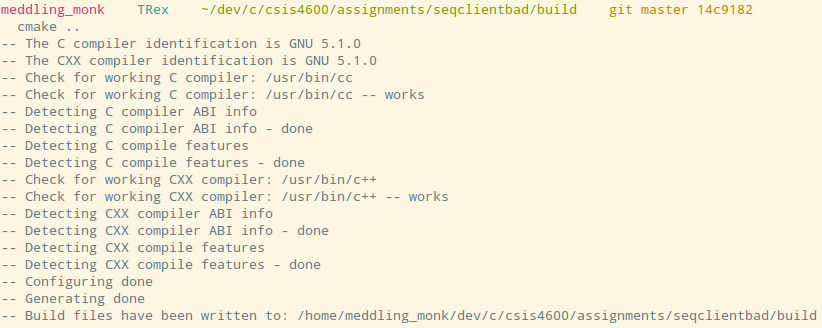
\includegraphics[width=1\linewidth]{./images/26}
	\caption[seqclientbad_cmake_prep]{\mintinline{c}{seqclientbad} CMake Metabuild}
	\label{fig:26}
\end{figure}
\begin{figure}[H]
	\centering
	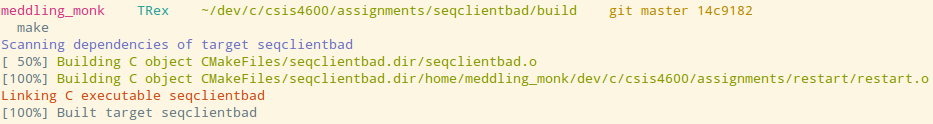
\includegraphics[width=1\linewidth]{./images/27}
	\caption[seqclientbad_make_build]{\mintinline{c}{seqclientbad} UNIX make}
	\label{fig:27}
\end{figure}
\subsection{Run}
To demonstrate \mintinline{c}{seqserverbad} and \mintinline{c}{seqclientbad}, they both will be loaded into GDB, and processed at each critical step.
\begin{figure}[H]
	\centering
	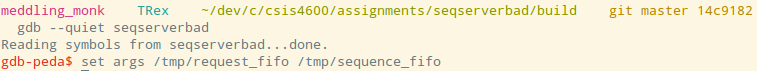
\includegraphics[width=1\linewidth]{./images/24}
	\caption[preparing_gdb_seqserver]{Preparing GDB with \mintinline{c}{seqserverbad}}
	\label{fig:28}
\end{figure}
Once \mintinline{c}{seqserverbad} has verified its argument count, it will create the FIFOs for reading requests and writing sequences.
After the FIFOs are made, it will block on read, waiting for a client to write a character to the request FIFO.
\begin{figure}[H]
	\centering
	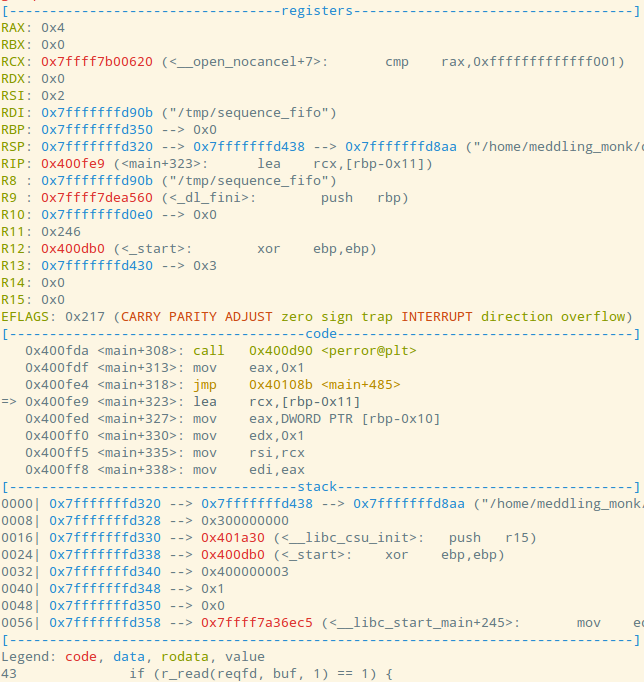
\includegraphics[width=1\linewidth]{./images/25}
	\caption[read_request_fifo]{Blocking on read of the request FIFO}
	\label{fig:29}
\end{figure}
Since the server has been started, and is waiting for requests, the client can be loaded into GDB, and requests can begin.
\begin{figure}[H]
	\centering
	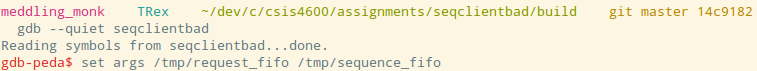
\includegraphics[width=1\linewidth]{./images/28}
	\caption[preparing_gdb_seqclient]{Preparing GDB with \mintinline{c}{seqclientbad}}
	\label{fig:30}
\end{figure}
\mintinline{c}{seqclientbad} will verify its argument count, just as \mintinline{c}{seqserverbad} did, and upon verification, it will open
the given FIFOs for writing requests and reading sequences. It's first request message will consist of one character: \mintinline{c}{'g'}.
\begin{figure}[H]
	\centering
	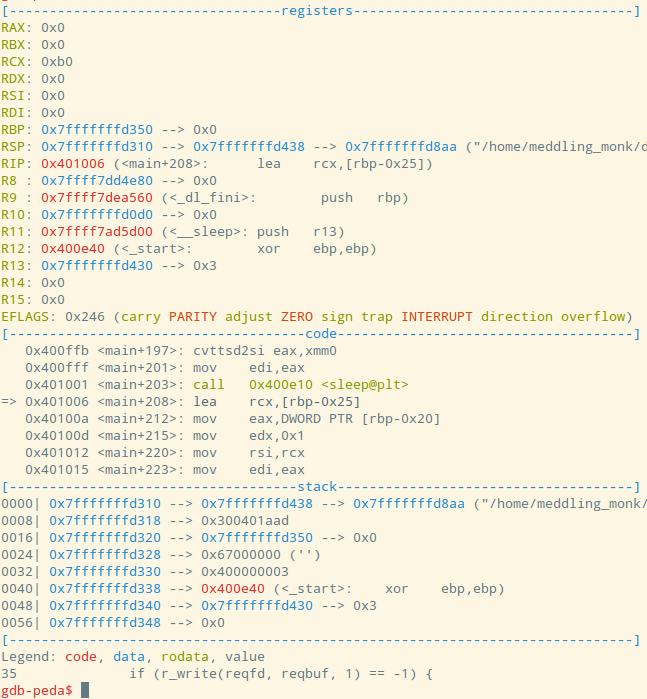
\includegraphics[width=1\linewidth]{./images/29}
	\caption[write_request_fifo]{\mintinline{c}{seqclient} writes \mintinline{c}{'g'} to the FIFO}
	\label{fig:31}
\end{figure}
\mintinline{c}{seqserverbad} will now read the \mintinline{c}{'g'} from \mintinline{c}{request_fifo}, and process the request.
Using GDB to print \mintinline{c}{buf}, it can be verified that \mintinline{c}{'g'} was indeed received from the FIFO.
\begin{figure}[H]
	\centering
	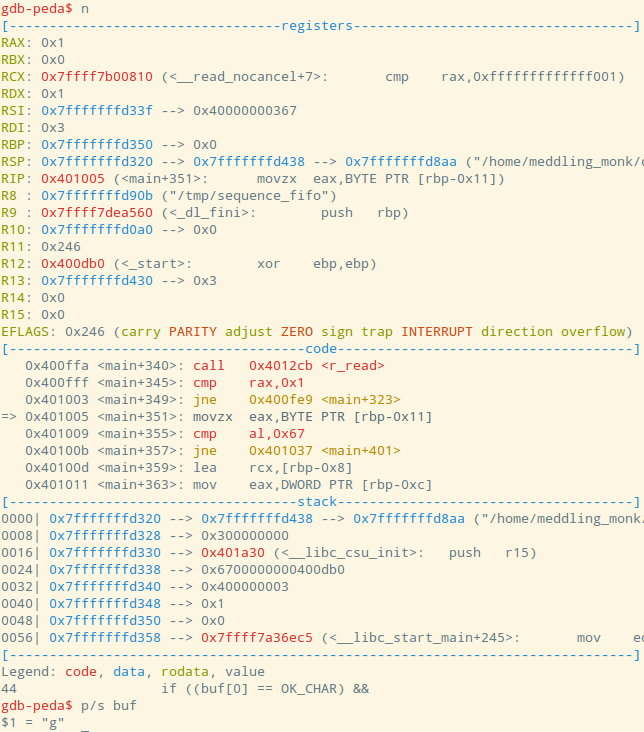
\includegraphics[width=1\linewidth]{./images/30}
	\caption[reading_char_from_request_fifo]{\mintinline{c}{seqserver} reads \mintinline{c}{'g'} from \mintinline{c}{request_fifo}}
	\label{fig:32}
\end{figure}
\mintinline{c}{seqserverbad} receipt of \mintinline{c}{'g'} also verifies that no error has occured in the communication. It is therefore ready 
to send its sequence over the \mintinline{c}{sequence_fifo} FIFO. The address of \mintinline{c}{sequence_fifo} can be viewed in register \mintinline{c}{R8}
at address \mintinline{c}{0x7fffffffd90b}. The character \mintinline{c}{'g'} can also be seen in the \mintinline{c}{RAX} register.
\begin{figure}[H]
	\centering
	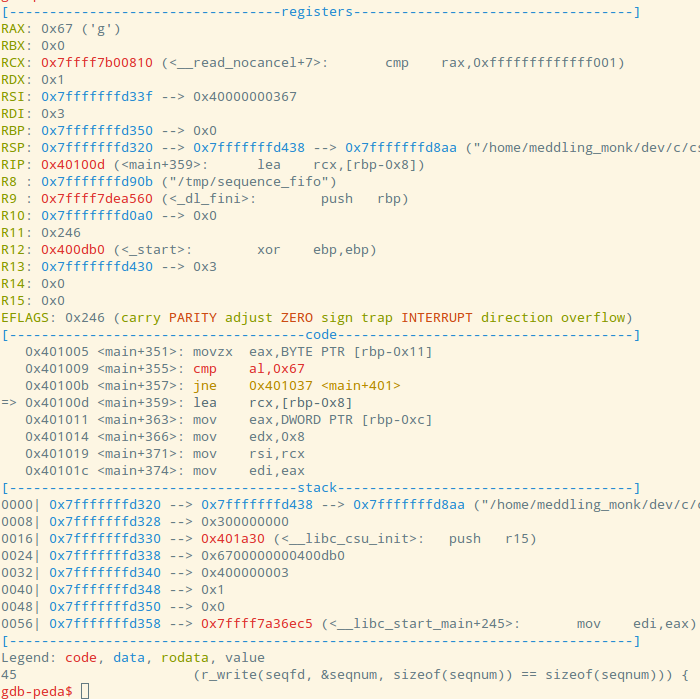
\includegraphics[width=1\linewidth]{./images/31}
	\caption[seqserverbad_sequence_fifo_write]{\mintinline{c}{seqserverbad} writes to \mintinline{c}{sequence_fifo}}
	\label{fig:33}
\end{figure}
Now that \mintinline{c}{seqserverbad} wrote to the \mintinline{c}{sequence_fifo}, \mintinline{c}{seqclientbad} can read its sequence number.
Printing \mintinline{c}{seqnum} as a decimal will reveal that 1 was indeed recieved, and the IPC executed across both FIFOs successfully.
\begin{figure}[H]
	\centering
	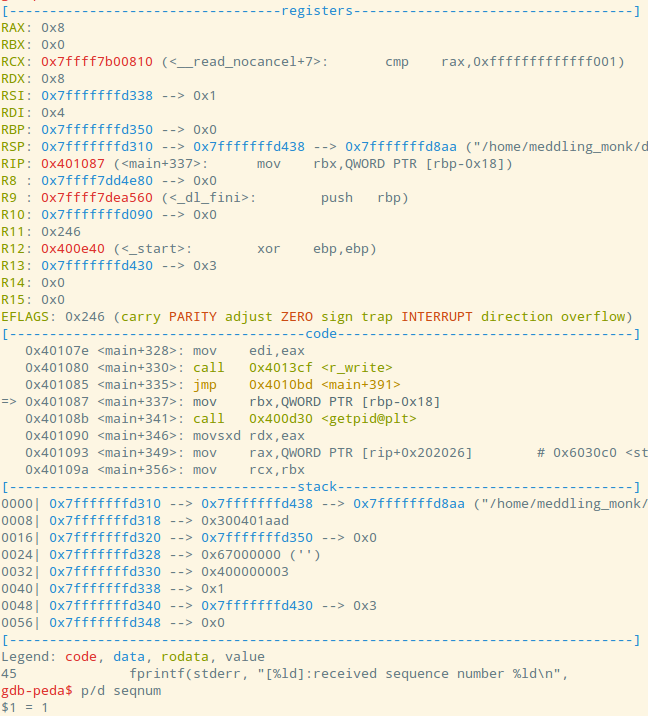
\includegraphics[width=1\linewidth]{./images/32}
	\caption[seqclientbad_sequence_fifo_read]{\mintinline{c}{seqclientbad} reads integer from \mintinline{c}{sequence_fifo}}
	\label{fig:34}
\end{figure}
\end{document}